\section{Symmetric Alice and Bob}
\textit{In this exercise, the flows between Alice and Bob are symmetric, similar to the discussions in class, meaning that each source provides a throughput of R to the system. This means that the system load at any point will be 2R. The task is to give derive the analytical expressions for the throughput for the case of not using network coding and the case of using network coding in the presence of a Medium Access Control (MAC) mechanism that provides fair access to the channel. Assume no losses occur in the different communication channels.}

\subsection{Exercise 1: Throughput Without Network Coding}
\textit{It is recommended to attack this problem in three stages. First, identify the three key regions of operation when not using network coding justifying your answer. Second, derive analytical expressions for the total system throughput, i.e., the addition of the end-to-end throughput of the connection from Alice to Bob and from Bob to Alice, versus the system load (2R). Finally, plot the total system throughput versus the system load.}\\

In the case without network coding the Relay sends the double amount of data compared to Alice and Bob until the maximum capacity is reached which is 0.5 R with a $50 \%$ of the load system, where A and B are sending $\dfrac{1}{4}R$. After this point the throughput will drop until $\dfrac{1}{3} R $ with a corresponding load of $66 \%$. After this point the throughput will stay stable at that value. To have a better understanding a plot (\figref{fig:throughput_WNC}) of the throughput vs the load of the system is made.
\begin{figure}[!h]
  \centering
  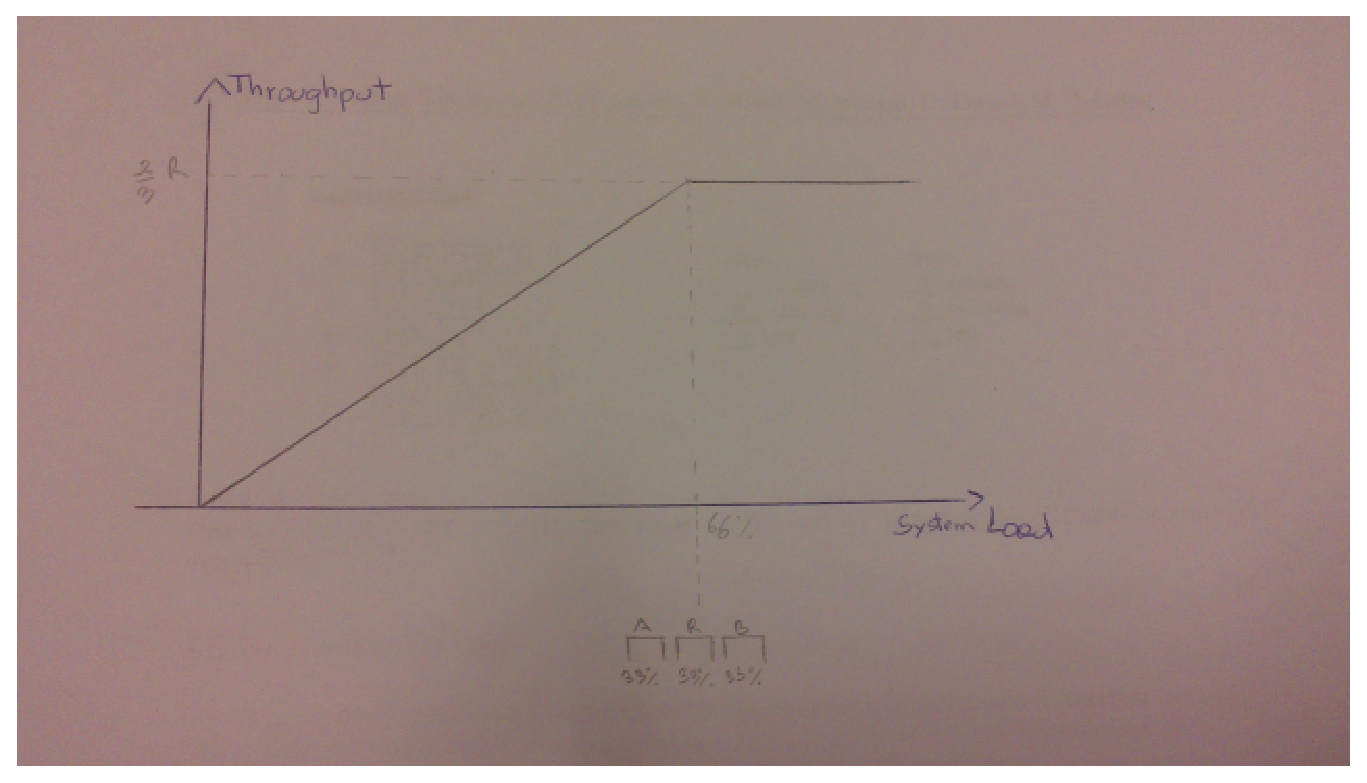
\includegraphics[width=15cm]{throughput_WNC.eps}
  \caption{throughput without NC}
  \label{fig:throughput_WNC}
\end{figure}

\subsection{Exercise 2: Throughput With Network Coding}
\textit{Repeat the steps of the previous question but using inter-session network coding at the relay. How many regions of operations are there and why?}\\

For the Network Coding the scenario is a bit different. The relays in this case sends the same amount of data as Alice and Bob. The throughput will grow until the maximum capacity is reached ($\dfrac{2}{3} R $), since each node is able to send $\dfrac{1}{3} R $ and it will stay stable with a $66 \%$ of the system load.  

\begin{figure}[!h]
  \centering
  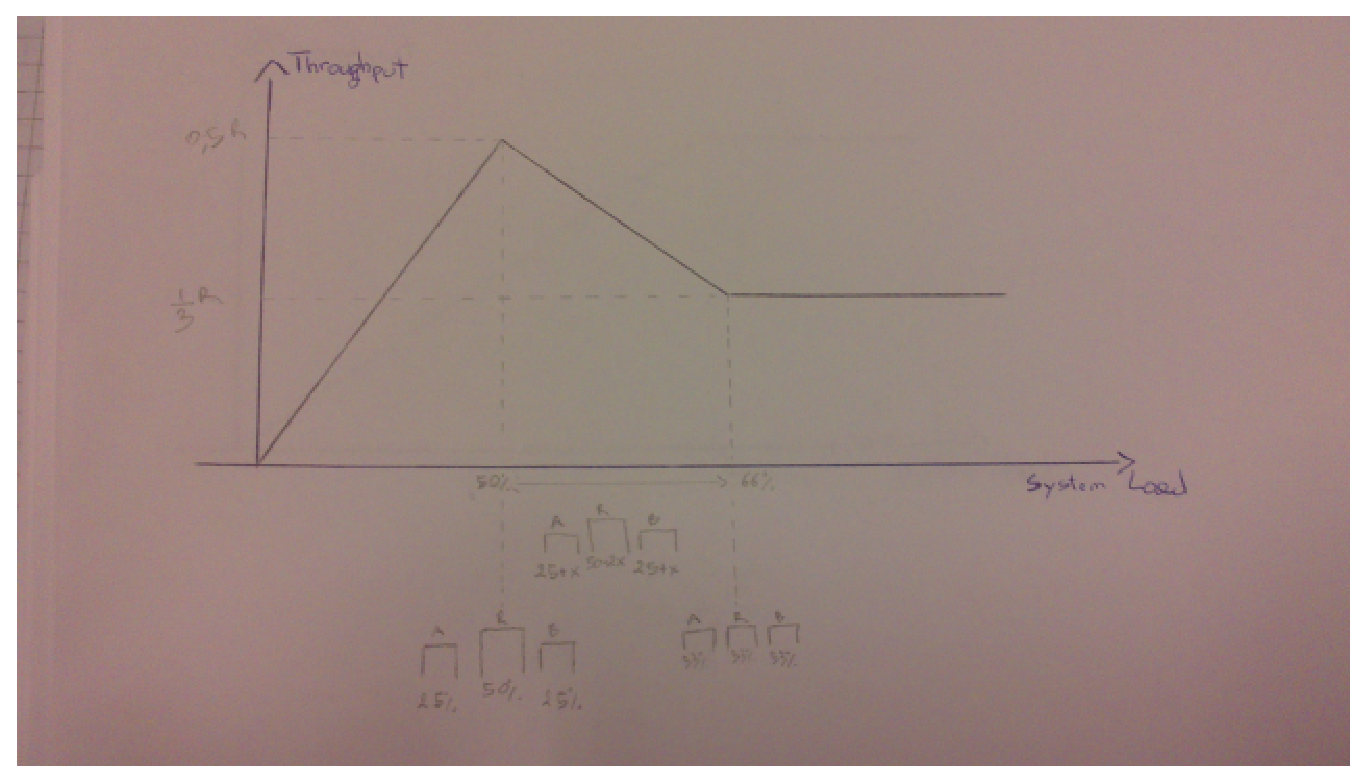
\includegraphics[width=15cm]{throughput_NC.eps}
  \caption{throughput with NC}
  \label{fig:throughput_NC}
\end{figure}
